\documentclass[]{book}
\usepackage{lmodern}
\usepackage{amssymb,amsmath}
\usepackage{ifxetex,ifluatex}
\usepackage{fixltx2e} % provides \textsubscript
\ifnum 0\ifxetex 1\fi\ifluatex 1\fi=0 % if pdftex
  \usepackage[T1]{fontenc}
  \usepackage[utf8]{inputenc}
\else % if luatex or xelatex
  \ifxetex
    \usepackage{mathspec}
  \else
    \usepackage{fontspec}
  \fi
  \defaultfontfeatures{Ligatures=TeX,Scale=MatchLowercase}
\fi
% use upquote if available, for straight quotes in verbatim environments
\IfFileExists{upquote.sty}{\usepackage{upquote}}{}
% use microtype if available
\IfFileExists{microtype.sty}{%
\usepackage[]{microtype}
\UseMicrotypeSet[protrusion]{basicmath} % disable protrusion for tt fonts
}{}
\PassOptionsToPackage{hyphens}{url} % url is loaded by hyperref
\usepackage[unicode=true]{hyperref}
\hypersetup{
            pdftitle={Merck-Data Mine Documentation},
            pdfauthor={Merck and Data Mine Corporate Partnership Team},
            pdfborder={0 0 0},
            breaklinks=true}
\urlstyle{same}  % don't use monospace font for urls
\usepackage{natbib}
\bibliographystyle{apalike}
\usepackage{color}
\usepackage{fancyvrb}
\newcommand{\VerbBar}{|}
\newcommand{\VERB}{\Verb[commandchars=\\\{\}]}
\DefineVerbatimEnvironment{Highlighting}{Verbatim}{commandchars=\\\{\}}
% Add ',fontsize=\small' for more characters per line
\usepackage{framed}
\definecolor{shadecolor}{RGB}{248,248,248}
\newenvironment{Shaded}{\begin{snugshade}}{\end{snugshade}}
\newcommand{\KeywordTok}[1]{\textcolor[rgb]{0.13,0.29,0.53}{\textbf{#1}}}
\newcommand{\DataTypeTok}[1]{\textcolor[rgb]{0.13,0.29,0.53}{#1}}
\newcommand{\DecValTok}[1]{\textcolor[rgb]{0.00,0.00,0.81}{#1}}
\newcommand{\BaseNTok}[1]{\textcolor[rgb]{0.00,0.00,0.81}{#1}}
\newcommand{\FloatTok}[1]{\textcolor[rgb]{0.00,0.00,0.81}{#1}}
\newcommand{\ConstantTok}[1]{\textcolor[rgb]{0.00,0.00,0.00}{#1}}
\newcommand{\CharTok}[1]{\textcolor[rgb]{0.31,0.60,0.02}{#1}}
\newcommand{\SpecialCharTok}[1]{\textcolor[rgb]{0.00,0.00,0.00}{#1}}
\newcommand{\StringTok}[1]{\textcolor[rgb]{0.31,0.60,0.02}{#1}}
\newcommand{\VerbatimStringTok}[1]{\textcolor[rgb]{0.31,0.60,0.02}{#1}}
\newcommand{\SpecialStringTok}[1]{\textcolor[rgb]{0.31,0.60,0.02}{#1}}
\newcommand{\ImportTok}[1]{#1}
\newcommand{\CommentTok}[1]{\textcolor[rgb]{0.56,0.35,0.01}{\textit{#1}}}
\newcommand{\DocumentationTok}[1]{\textcolor[rgb]{0.56,0.35,0.01}{\textbf{\textit{#1}}}}
\newcommand{\AnnotationTok}[1]{\textcolor[rgb]{0.56,0.35,0.01}{\textbf{\textit{#1}}}}
\newcommand{\CommentVarTok}[1]{\textcolor[rgb]{0.56,0.35,0.01}{\textbf{\textit{#1}}}}
\newcommand{\OtherTok}[1]{\textcolor[rgb]{0.56,0.35,0.01}{#1}}
\newcommand{\FunctionTok}[1]{\textcolor[rgb]{0.00,0.00,0.00}{#1}}
\newcommand{\VariableTok}[1]{\textcolor[rgb]{0.00,0.00,0.00}{#1}}
\newcommand{\ControlFlowTok}[1]{\textcolor[rgb]{0.13,0.29,0.53}{\textbf{#1}}}
\newcommand{\OperatorTok}[1]{\textcolor[rgb]{0.81,0.36,0.00}{\textbf{#1}}}
\newcommand{\BuiltInTok}[1]{#1}
\newcommand{\ExtensionTok}[1]{#1}
\newcommand{\PreprocessorTok}[1]{\textcolor[rgb]{0.56,0.35,0.01}{\textit{#1}}}
\newcommand{\AttributeTok}[1]{\textcolor[rgb]{0.77,0.63,0.00}{#1}}
\newcommand{\RegionMarkerTok}[1]{#1}
\newcommand{\InformationTok}[1]{\textcolor[rgb]{0.56,0.35,0.01}{\textbf{\textit{#1}}}}
\newcommand{\WarningTok}[1]{\textcolor[rgb]{0.56,0.35,0.01}{\textbf{\textit{#1}}}}
\newcommand{\AlertTok}[1]{\textcolor[rgb]{0.94,0.16,0.16}{#1}}
\newcommand{\ErrorTok}[1]{\textcolor[rgb]{0.64,0.00,0.00}{\textbf{#1}}}
\newcommand{\NormalTok}[1]{#1}
\usepackage{longtable,booktabs}
% Fix footnotes in tables (requires footnote package)
\IfFileExists{footnote.sty}{\usepackage{footnote}\makesavenoteenv{long table}}{}
\usepackage{graphicx,grffile}
\makeatletter
\def\maxwidth{\ifdim\Gin@nat@width>\linewidth\linewidth\else\Gin@nat@width\fi}
\def\maxheight{\ifdim\Gin@nat@height>\textheight\textheight\else\Gin@nat@height\fi}
\makeatother
% Scale images if necessary, so that they will not overflow the page
% margins by default, and it is still possible to overwrite the defaults
% using explicit options in \includegraphics[width, height, ...]{}
\setkeys{Gin}{width=\maxwidth,height=\maxheight,keepaspectratio}
\IfFileExists{parskip.sty}{%
\usepackage{parskip}
}{% else
\setlength{\parindent}{0pt}
\setlength{\parskip}{6pt plus 2pt minus 1pt}
}
\setlength{\emergencystretch}{3em}  % prevent overfull lines
\providecommand{\tightlist}{%
  \setlength{\itemsep}{0pt}\setlength{\parskip}{0pt}}
\setcounter{secnumdepth}{5}
% Redefines (sub)paragraphs to behave more like sections
\ifx\paragraph\undefined\else
\let\oldparagraph\paragraph
\renewcommand{\paragraph}[1]{\oldparagraph{#1}\mbox{}}
\fi
\ifx\subparagraph\undefined\else
\let\oldsubparagraph\subparagraph
\renewcommand{\subparagraph}[1]{\oldsubparagraph{#1}\mbox{}}
\fi

% set default figure placement to htbp
\makeatletter
\def\fps@figure{htbp}
\makeatother

\usepackage{booktabs}
\usepackage{amsthm}
\makeatletter
\def\thm@space@setup{%
  \thm@preskip=8pt plus 2pt minus 4pt
  \thm@postskip=\thm@preskip
}
\makeatother

\title{Merck-Data Mine Documentation}
\author{Merck and Data Mine Corporate Partnership Team}
\date{2020-07-29}

\begin{document}
\maketitle

{
\setcounter{tocdepth}{1}
\tableofcontents
}
\chapter{Introduction}\label{introduction}

This book will serve as tutorial based documentation for the Merck -
Data Mine Coporate Partnership team for the 2020-2021 academic year.

\section{How to contribute}\label{how-to-contribute}

Contributing to this book is simple:

\subsection{Small changes and
additions}\label{small-changes-and-additions}

If you have a small change or addition you'd like to make to the book,
the easiest way to quickly contribute would be the following method.

\begin{enumerate}
\def\labelenumi{\arabic{enumi}.}
\item
  Navigate to the page or section that needs to be edited
\item
  Click on the ``Edit'' button towards the upper left side of the page:
  
\includegraphics{images/edit_button.png}
\item
  You'll be presented with the respective RMarkdown file. Make your
  modifications.
\item
  In the ``Commit changes'' box, select the radio button that says
  \emph{Create a \textbf{new branch} for this commit and start a pull
  request.} Give your pull request a title and a detailed description.
  Name the new branch, and click on ``Propose file change''.
\item
  You've successfully submitted a pull request. Our team will review and
  merge the request shortly thereafter.
\end{enumerate}

\subsection{Larger changes or
additions}\label{larger-changes-or-additions}

If you have larger changes or additions you'd like to make to the book,
the easiest way is to edit the contents of the book on your local
machine.

\subsubsection{\texorpdfstring{Using \texttt{git} in the
terminal}{Using git in the terminal}}\label{using-git-in-the-terminal}

\begin{enumerate}
\def\labelenumi{\arabic{enumi}.}
\tightlist
\item
  Setup \texttt{git} following the directions
  \protect\hyperlink{git-install}{here}.
\item
  Start by opening up a terminal and
  \protect\hyperlink{configure-git}{configuring \texttt{git} to work
  with GitHub}.
\item
  Navigate to the directory in which you would like to clone
  the-examples-book repository. For example, if I wanted to clone the
  repository in my \texttt{\textasciitilde{}/projects} folder, I'd first
  execute: \texttt{cd\ \textasciitilde{}/projects}.
\item
  \protect\hyperlink{git-clone-repository}{Clone the repository}. In
  this example, let's assume I've cloned the repository into my
  \texttt{\textasciitilde{}/projects} folder.
\item
  Navigate into the project folder:
\end{enumerate}

\begin{Shaded}
\begin{Highlighting}[]
\BuiltInTok{cd}\NormalTok{ ~/projects/the-examples-book}
\end{Highlighting}
\end{Shaded}

\begin{enumerate}
\def\labelenumi{\arabic{enumi}.}
\setcounter{enumi}{5}
\tightlist
\item
  At this point in time your current branch should be the
  \texttt{master} branch. You can verify by running:
\end{enumerate}

\begin{Shaded}
\begin{Highlighting}[]
\FunctionTok{git}\NormalTok{ branch}
\end{Highlighting}
\end{Shaded}

\textbf{Note:} The highlighted branch starting with ``*" is the current
branch.

or if you'd like just the name of the branch:

\begin{Shaded}
\begin{Highlighting}[]
\FunctionTok{git}\NormalTok{ rev-parse --abbrev-ref HEAD}
\end{Highlighting}
\end{Shaded}

\begin{enumerate}
\def\labelenumi{\arabic{enumi}.}
\setcounter{enumi}{6}
\item
  \protect\hyperlink{git-create-new-branch}{Create a new branch} with
  whatever name you'd like, and check that branch out. For example,
  \texttt{fix-spelling-errors-01}.
\item
  Open up RStudio. In the ``Files'' tab in RStudio, navigate to the
  repository. In this example, we would navigate to
  \texttt{/Users/kamstut/Documents/GitHub/the-examples-book}. Click on
  the ``More'' dropdown and select ``Set As Working Directory''.
\item
  If you do not already have \texttt{renv} installed, install it by
  running the following commands in the console:
\end{enumerate}

\begin{Shaded}
\begin{Highlighting}[]
\KeywordTok{install.packages}\NormalTok{(}\StringTok{"renv"}\NormalTok{)}
\end{Highlighting}
\end{Shaded}

\begin{enumerate}
\def\labelenumi{\arabic{enumi}.}
\setcounter{enumi}{9}
\tightlist
\item
  Restore the environment by running the following commands in the
  console:
\end{enumerate}

\begin{Shaded}
\begin{Highlighting}[]
\NormalTok{renv}\OperatorTok{::}\KeywordTok{restore}\NormalTok{()}
\end{Highlighting}
\end{Shaded}

\begin{enumerate}
\def\labelenumi{\arabic{enumi}.}
\setcounter{enumi}{10}
\tightlist
\item
  In order to compile this book, you must have LaTeX installed. The
  easiest way to accomplish this is to run the following in the R
  console:
\end{enumerate}

\begin{Shaded}
\begin{Highlighting}[]
\KeywordTok{install.packages}\NormalTok{(}\StringTok{"tinytex"}\NormalTok{)}
\KeywordTok{library}\NormalTok{(tinytex)}
\NormalTok{tinytex}\OperatorTok{::}\KeywordTok{install_tinytex}\NormalTok{()}
\end{Highlighting}
\end{Shaded}

\begin{enumerate}
\def\labelenumi{\arabic{enumi}.}
\setcounter{enumi}{11}
\item
  In addition, make sure to install both \texttt{pandoc} and
  \texttt{pandoc-citeproc} by following the instructions
  \href{https://pandoc.org/installing.html}{here}.
\item
  Modify the \texttt{.Rmd} files to your liking.
\item
  Click the ``Knit'' button to compile the book. The resulting ``book''
  is within the ``docs'' folder.
\end{enumerate}

\textbf{Important note:} If at any point in time you receive an error
saying something similar to ``there is no package called
\texttt{my\_package}, simply install the missing package, and try to
knit again:

\begin{Shaded}
\begin{Highlighting}[]
\KeywordTok{install.packages}\NormalTok{(}\StringTok{"my_package"}\NormalTok{)}
\KeywordTok{library}\NormalTok{(my_package)}
\end{Highlighting}
\end{Shaded}

\begin{enumerate}
\def\labelenumi{\arabic{enumi}.}
\setcounter{enumi}{14}
\tightlist
\item
  To test the book out, navigate to the ``docs'' folder and open the
  \texttt{index.html} in the browser of your choice.
\item
  When you are happy with the modifications you've made,
  \protect\hyperlink{git-commit-changes}{commit your changes} to the
  repository.
\item
  You can continue to make modifications and commit your changes
  locally. When you are ready, you can
  \protect\hyperlink{git-push-local-commits}{push your branch} to the
  remote repository (github.com).
\item
  At this point in time, you can confirm that the branch has been
  succesfully pushed to github.com by navigating to the repository on
  github, and click on the ``branches'' tab:
\end{enumerate}

\begin{figure}
\centering
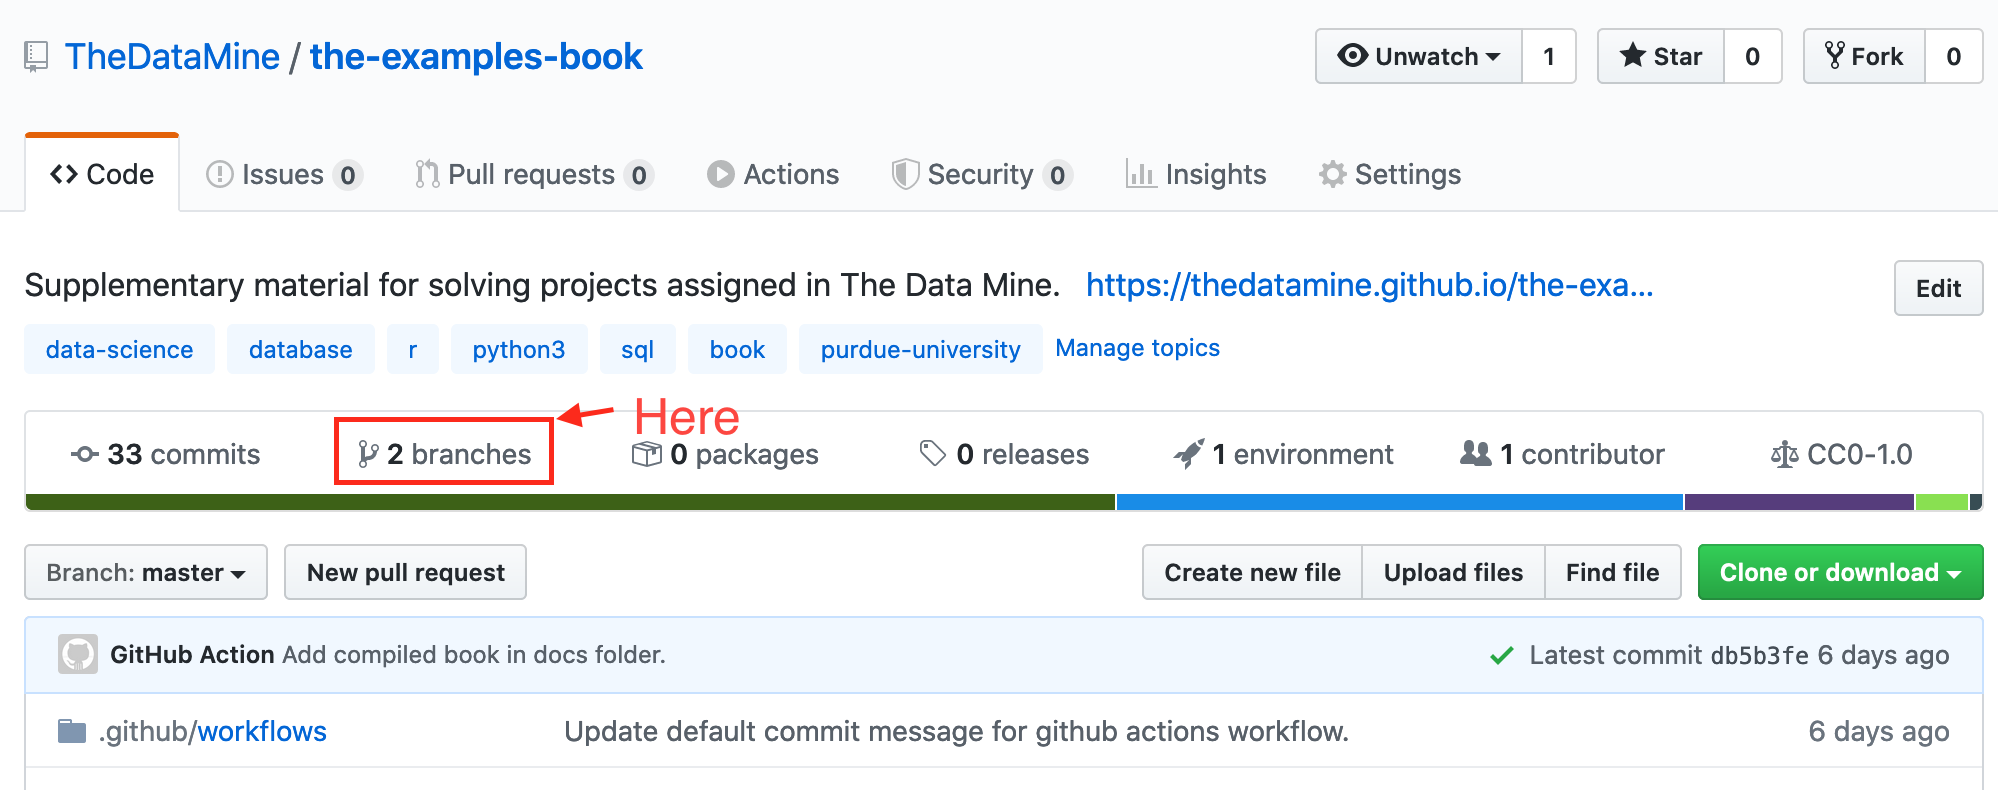
\includegraphics{./images/gh-desktop-14.png}
\caption{}
\end{figure}

\begin{enumerate}
\def\labelenumi{\arabic{enumi}.}
\setcounter{enumi}{18}
\tightlist
\item
  Next, \href{}{create a pull request}. Note that a ``Pull Request'' is
  a GitHub-specific concept. You cannot create a pull request using
  \texttt{git}. Navigate to the repository
  \url{https://github.com/thedatamine/the-examples-book}, and you should
  see a message asking if you'd like to create a pull request:
\end{enumerate}

\begin{figure}
\centering
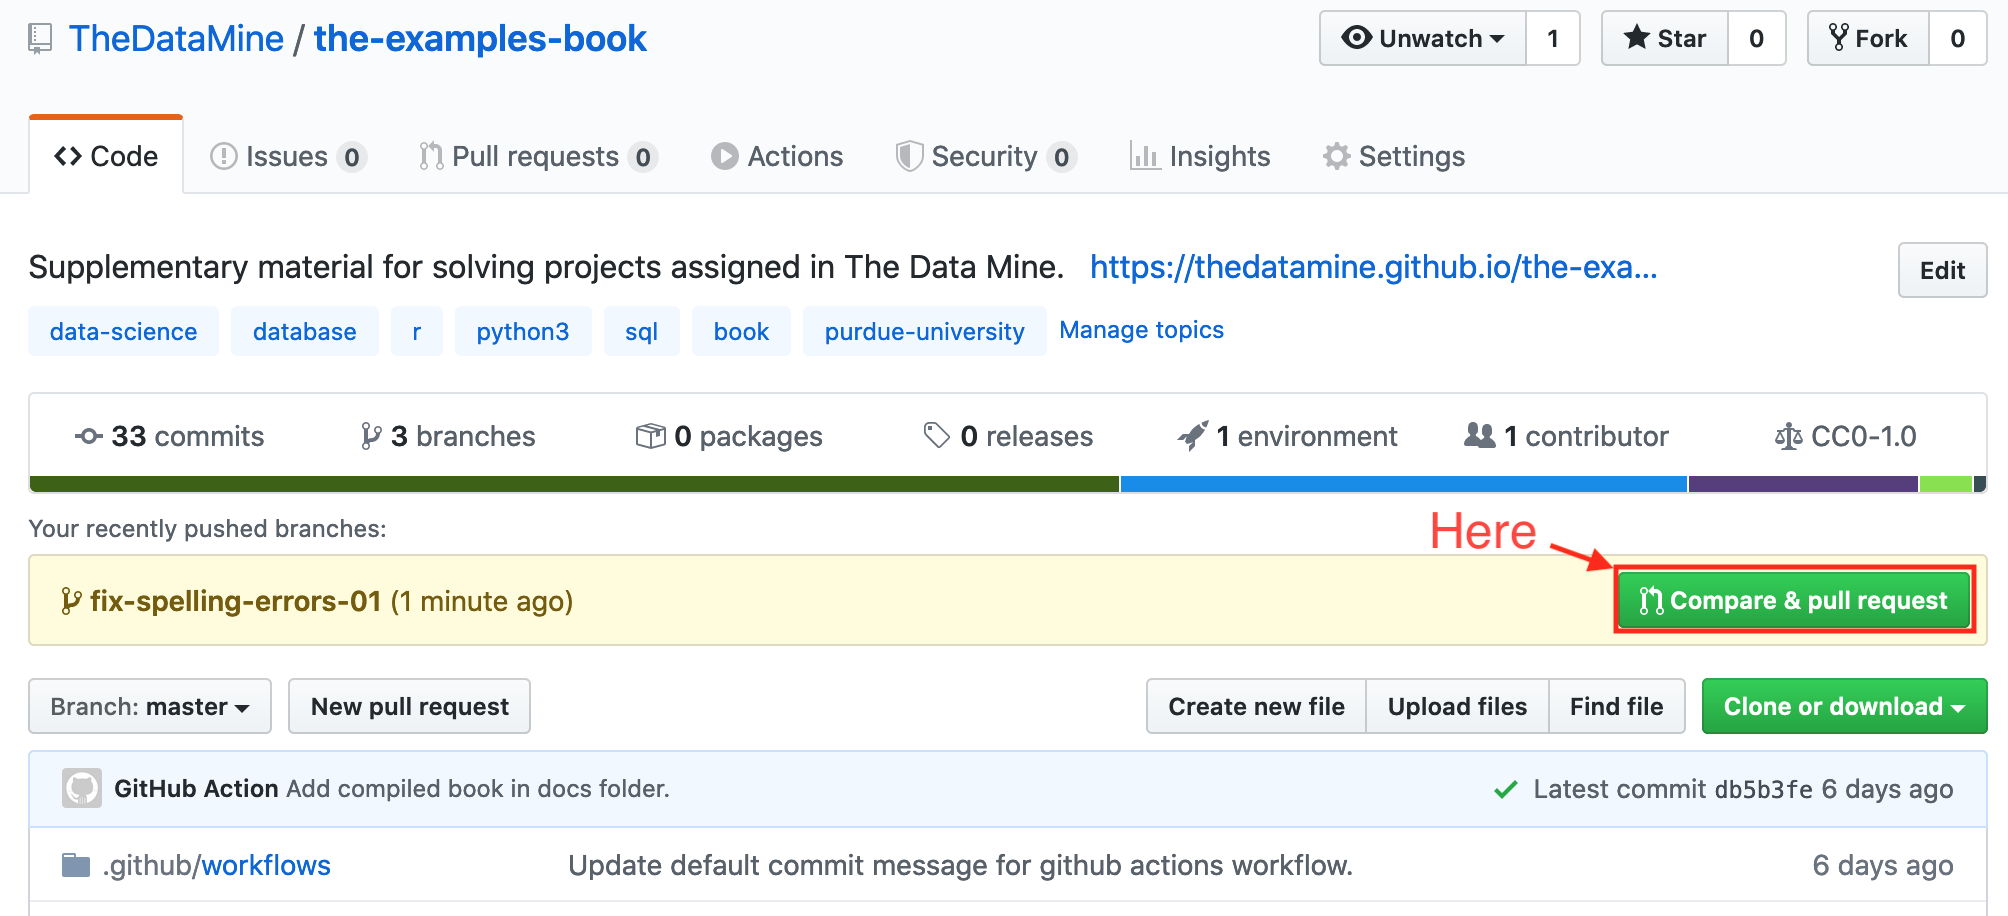
\includegraphics{./images/pr-01.png}
\caption{}
\end{figure}

\begin{enumerate}
\def\labelenumi{\arabic{enumi}.}
\setcounter{enumi}{19}
\item
  Leave a detailed comment about what you've modified or added to the
  book. You can click on ``Preview'' to see what your comment will look
  like.
  \href{https://help.github.com/en/github/writing-on-github/basic-writing-and-formatting-syntax}{GitHub's
  markdown} applies here. Once satisfied, click ``Create pull request''.
\item
  At this point in time, the repository owners will receive a
  notification and will check and potentially merge the changes into the
  \texttt{master} branch.
\end{enumerate}

\subsubsection{Using GitHub Desktop}\label{using-github-desktop}

\begin{enumerate}
\def\labelenumi{\arabic{enumi}.}
\tightlist
\item
  Setup GitHub Desktop following the directions
  \protect\hyperlink{github-desktop-install}{here}.
\item
  When you are presented with the following screen, select ``Clone a
  Repository from the Internet\ldots{}'':
\end{enumerate}

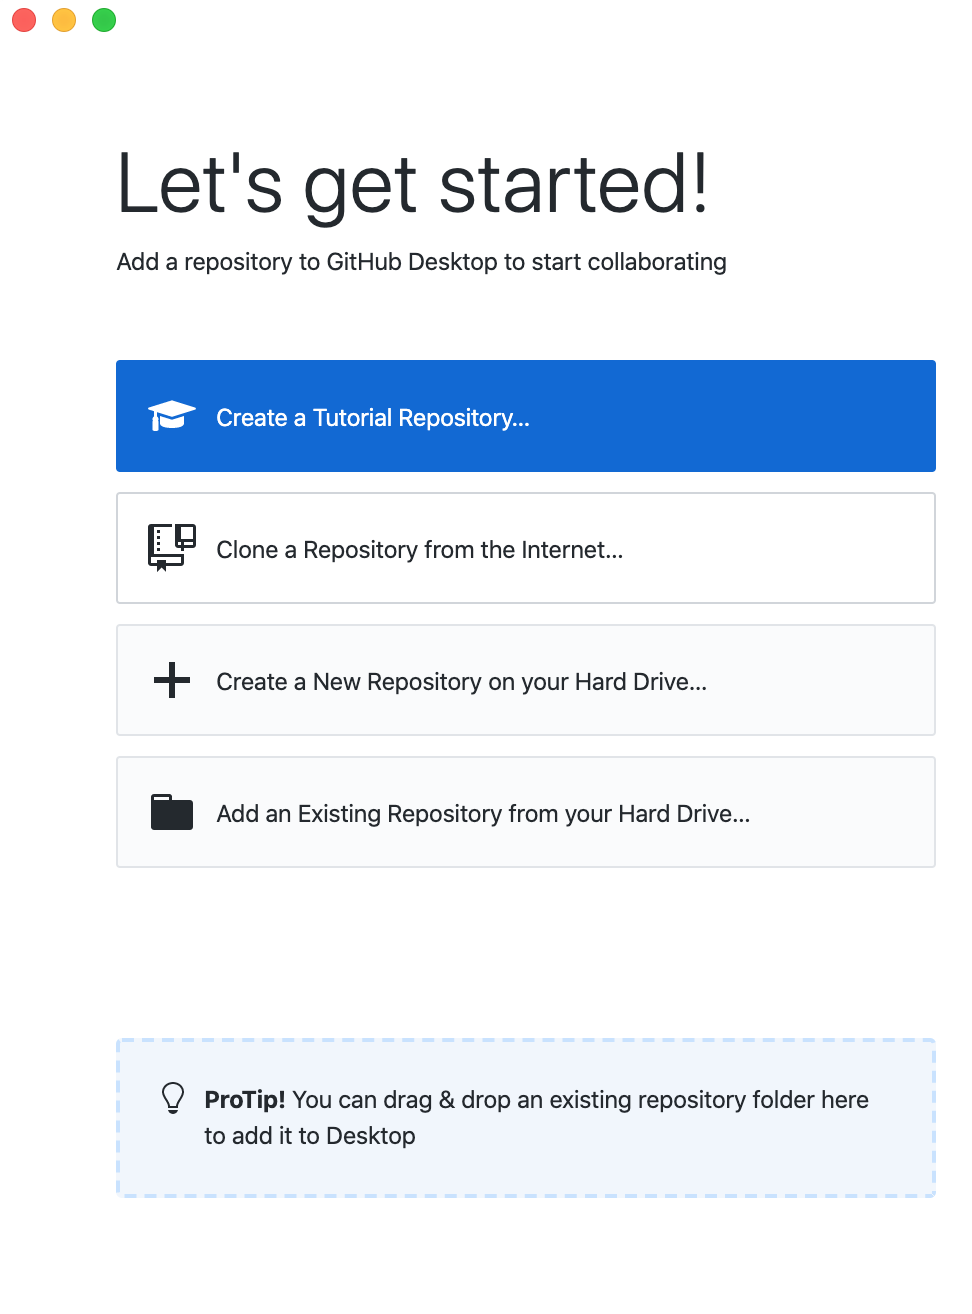
\includegraphics{./images/gh-desktop-03.png} 3. Click on the ``URL''
tab:

\begin{figure}
\centering
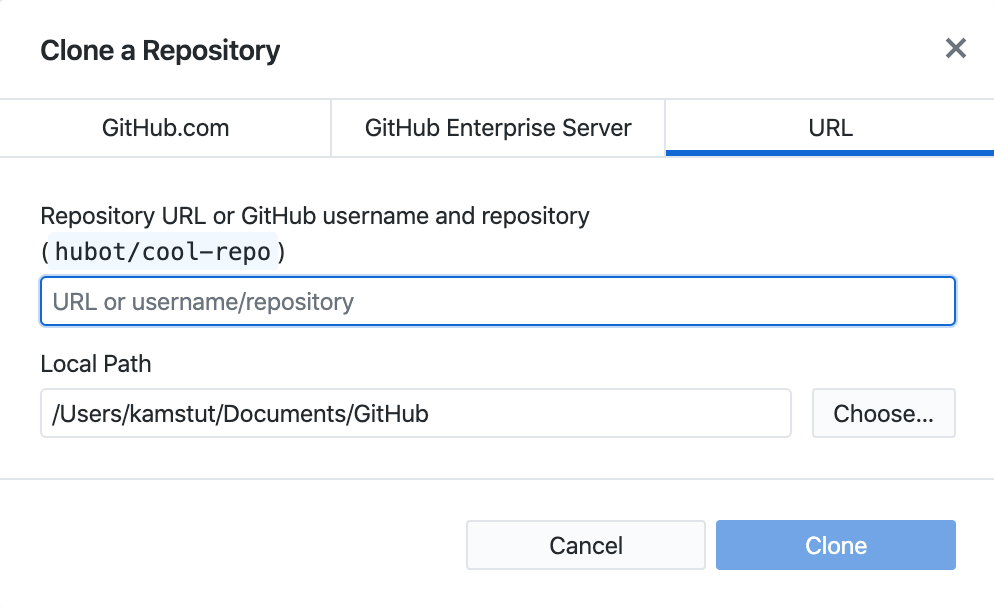
\includegraphics{./images/gh-desktop-04.png}
\caption{}
\end{figure}

\begin{enumerate}
\def\labelenumi{\arabic{enumi}.}
\setcounter{enumi}{3}
\tightlist
\item
  In the first field, enter ``TheDataMine/the-examples-book''. This is
  the repository for this book.
\item
  In the second field, enter the location in which you'd like the
  repository to be cloned to. In this example, the repository will be
  cloned into \texttt{/Users/kamstut/Documents/GitHub}. The result will
  be a new folder called \texttt{the-examples-book} in
  \texttt{/Users/kamstut/Documents/GitHub}.
\item
  Click ``Clone''.
\item
  Upon completion, you will be presented with a screen similar to this:
\end{enumerate}

\begin{figure}
\centering
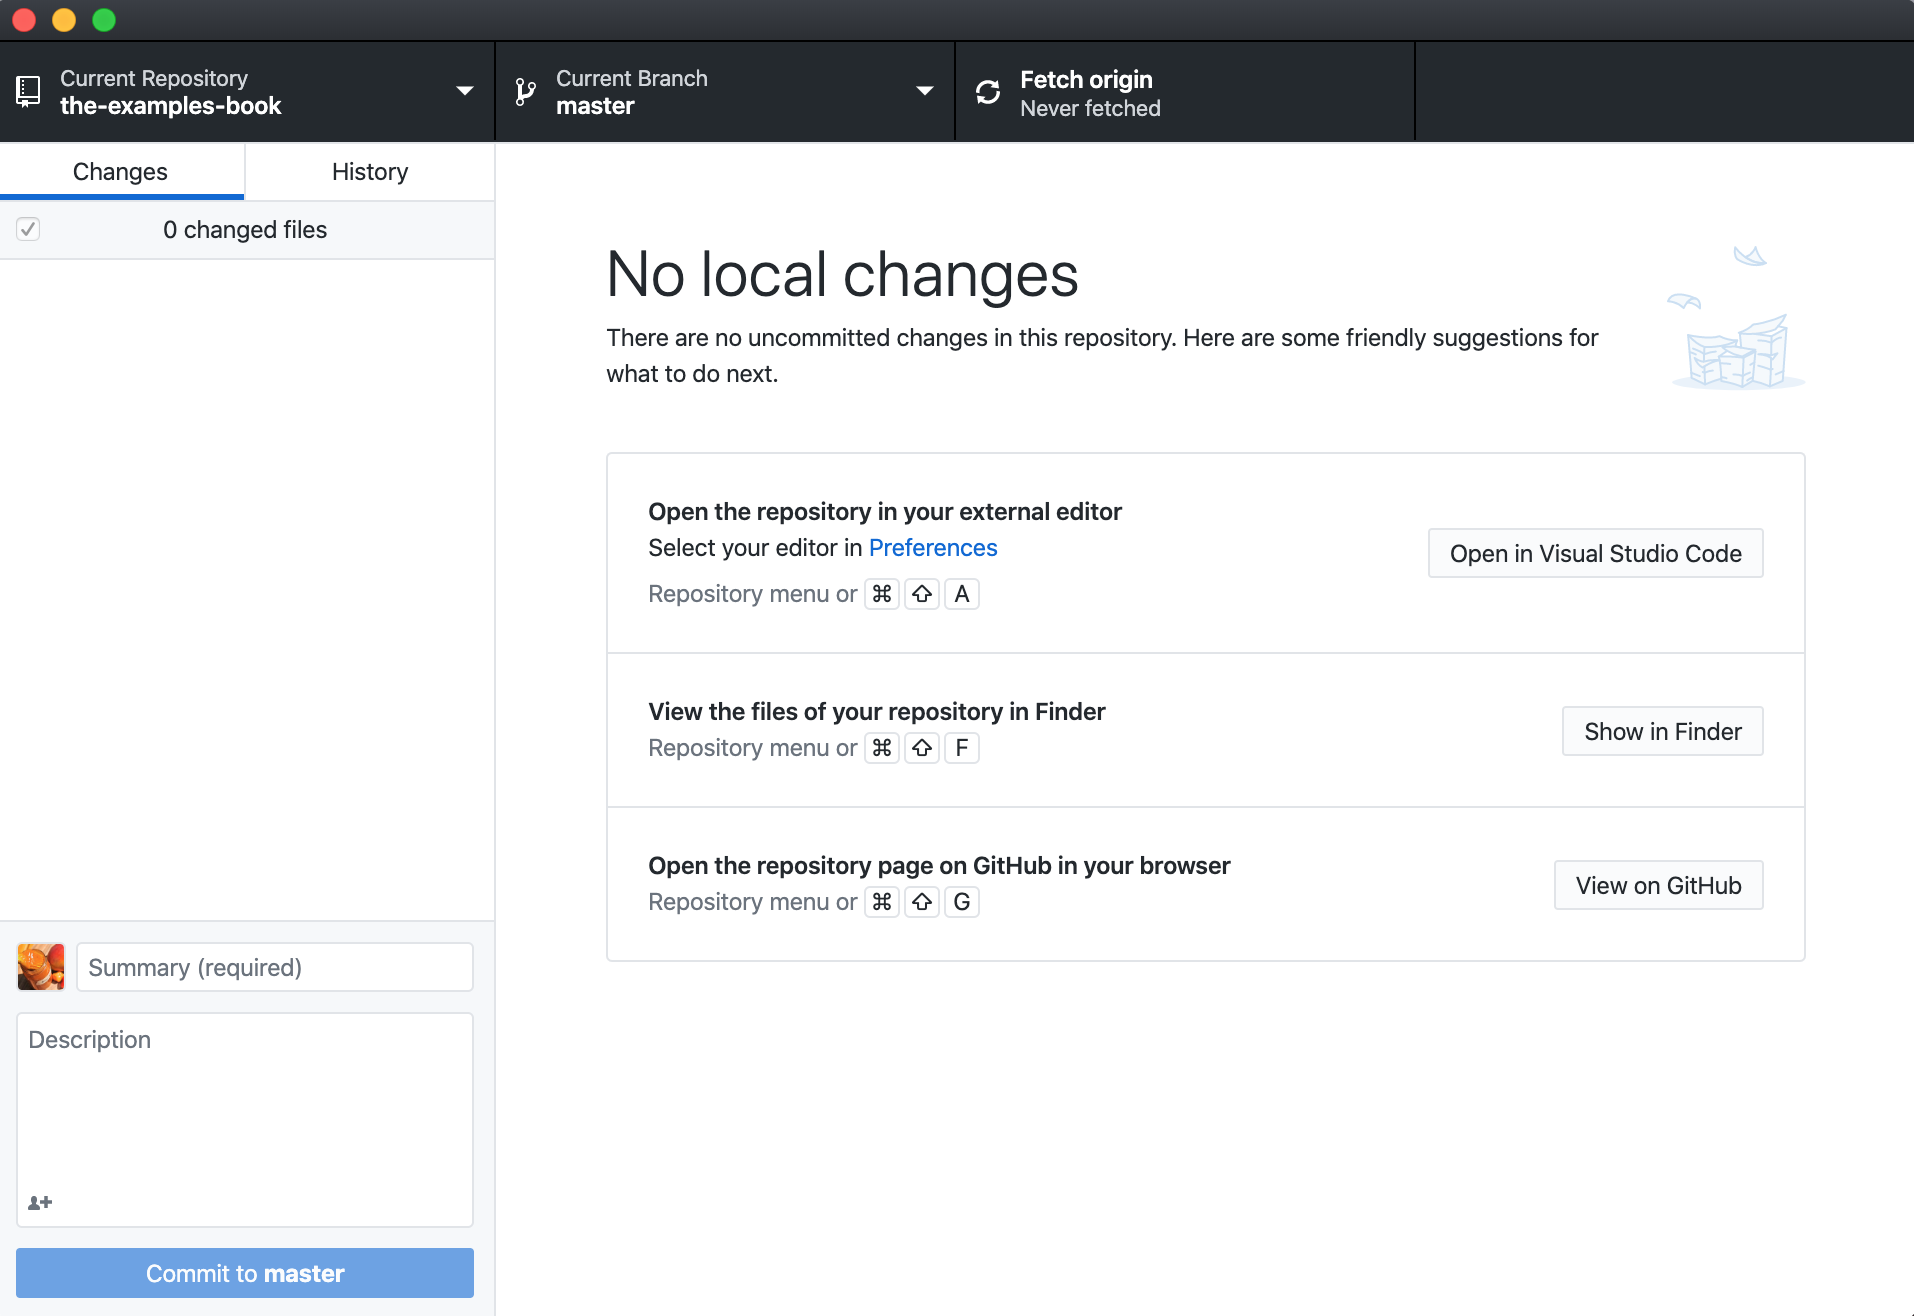
\includegraphics{./images/gh-desktop-05.png}
\caption{}
\end{figure}

\begin{enumerate}
\def\labelenumi{\arabic{enumi}.}
\setcounter{enumi}{7}
\tightlist
\item
  At this point in time, your current branch will be the \texttt{master}
  branch. \protect\hyperlink{github-desktop-create-new-branch}{Create a
  new branch} with whatever name you'd like. For example,
  \texttt{fix-spelling-errors-01}.
\item
  Open up RStudio. In the ``Files'' tab in RStudio, navigate to the
  repository. In this example, we would navigate to
  \texttt{/Users/kamstut/Documents/GitHub/the-examples-book}. Click on
  the ``More'' dropdown and select ``Set As Working Directory''.
\item
  If you do not already have \texttt{renv} installed, install it by
  running the following commands in the console:
\end{enumerate}

\begin{Shaded}
\begin{Highlighting}[]
\KeywordTok{install.packages}\NormalTok{(}\StringTok{"renv"}\NormalTok{)}
\end{Highlighting}
\end{Shaded}

\begin{enumerate}
\def\labelenumi{\arabic{enumi}.}
\setcounter{enumi}{10}
\tightlist
\item
  Restore the environment by running the following commands in the
  console:
\end{enumerate}

\begin{Shaded}
\begin{Highlighting}[]
\NormalTok{renv}\OperatorTok{::}\KeywordTok{restore}\NormalTok{()}
\end{Highlighting}
\end{Shaded}

\begin{enumerate}
\def\labelenumi{\arabic{enumi}.}
\setcounter{enumi}{11}
\tightlist
\item
  In order to compile this book, you must have LaTeX installed. The
  easiest way to accomplish this is to run the following in the R
  console:
\end{enumerate}

\begin{Shaded}
\begin{Highlighting}[]
\KeywordTok{install.packages}\NormalTok{(}\StringTok{"tinytex"}\NormalTok{)}
\KeywordTok{library}\NormalTok{(tinytex)}
\NormalTok{tinytex}\OperatorTok{::}\KeywordTok{install_tinytex}\NormalTok{()}
\end{Highlighting}
\end{Shaded}

\begin{enumerate}
\def\labelenumi{\arabic{enumi}.}
\setcounter{enumi}{12}
\item
  In addition, make sure to install both \texttt{pandoc} and
  \texttt{pandoc-citeproc} by following the instructions
  \href{https://pandoc.org/installing.html}{here}.
\item
  Modify the \texttt{.Rmd} files to your liking.
\item
  Click the ``Knit'' button to compile the book. The resulting ``book''
  is within the ``docs'' folder.
\end{enumerate}

\textbf{Important note:} If at any point in time you receive an error
saying something similar to ``there is no package called
\texttt{my\_package}, simply install the missing package, and try to
knit again:

\begin{Shaded}
\begin{Highlighting}[]
\KeywordTok{install.packages}\NormalTok{(}\StringTok{"my_package"}\NormalTok{)}
\KeywordTok{library}\NormalTok{(my_package)}
\end{Highlighting}
\end{Shaded}

\begin{enumerate}
\def\labelenumi{\arabic{enumi}.}
\setcounter{enumi}{15}
\tightlist
\item
  To test the book out, navigate to the ``docs'' folder and open the
  \texttt{index.html} in the browser of your choice.
\item
  When you are happy with the modifications you've made,
  \protect\hyperlink{github-desktop-commit-changes}{commit your changes}
  to the repository.
\item
  You can continue to make modifications and commit your changes
  locally. When you are ready, you can
  \protect\hyperlink{github-desktop-publish-branch}{publish your
  branch}:
\end{enumerate}

\begin{figure}
\centering
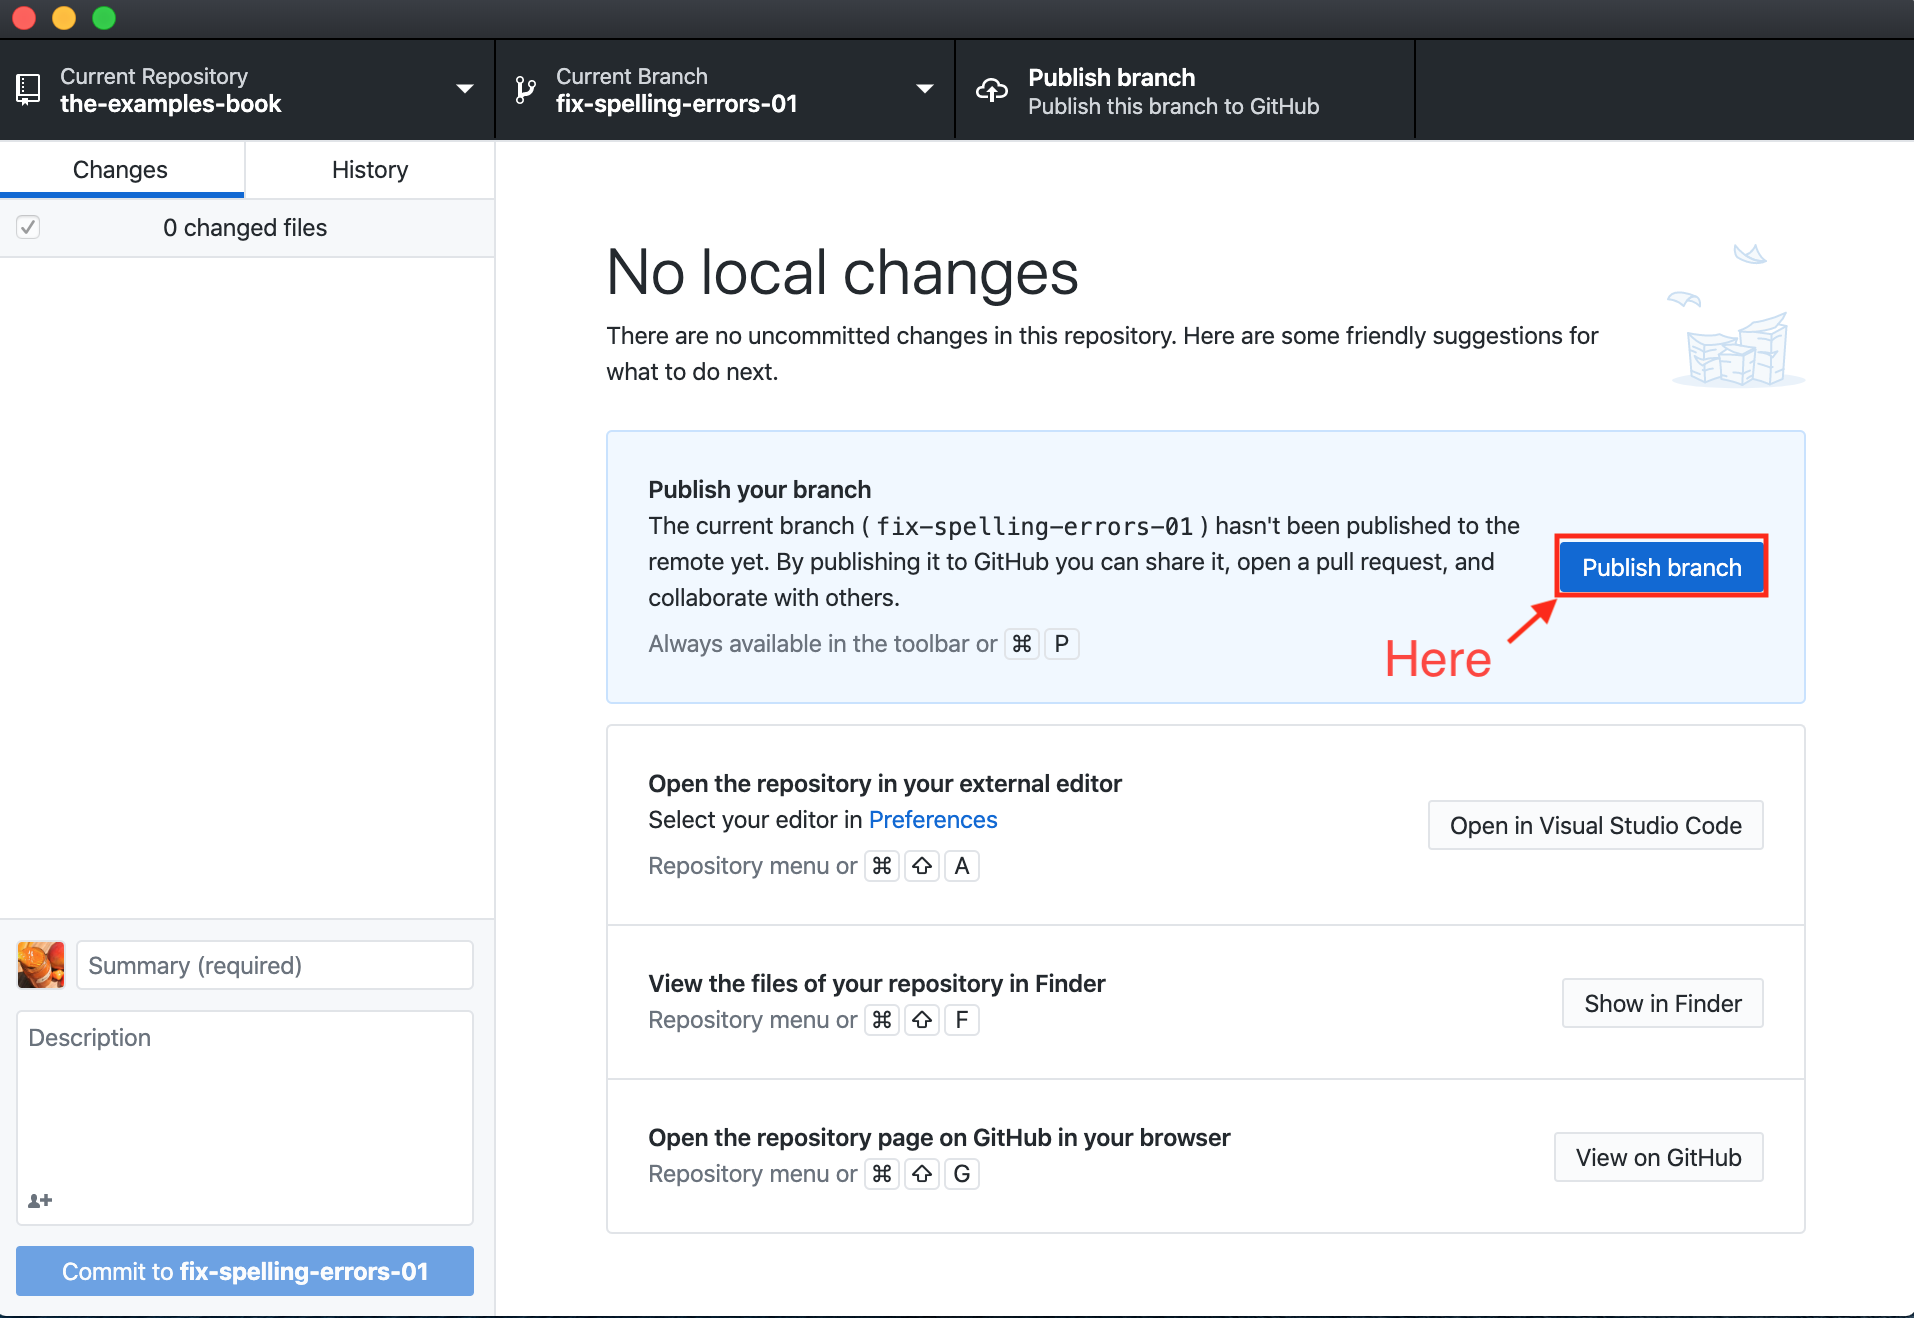
\includegraphics{./images/gh-desktop-13.png}
\caption{}
\end{figure}

\begin{enumerate}
\def\labelenumi{\arabic{enumi}.}
\setcounter{enumi}{18}
\tightlist
\item
  Upon publishing your branch, within GitHub Desktop, you'll be
  presented with the option to
  \protect\hyperlink{github-desktop-pull-request}{create a pull
  request}:
\end{enumerate}

\begin{figure}
\centering
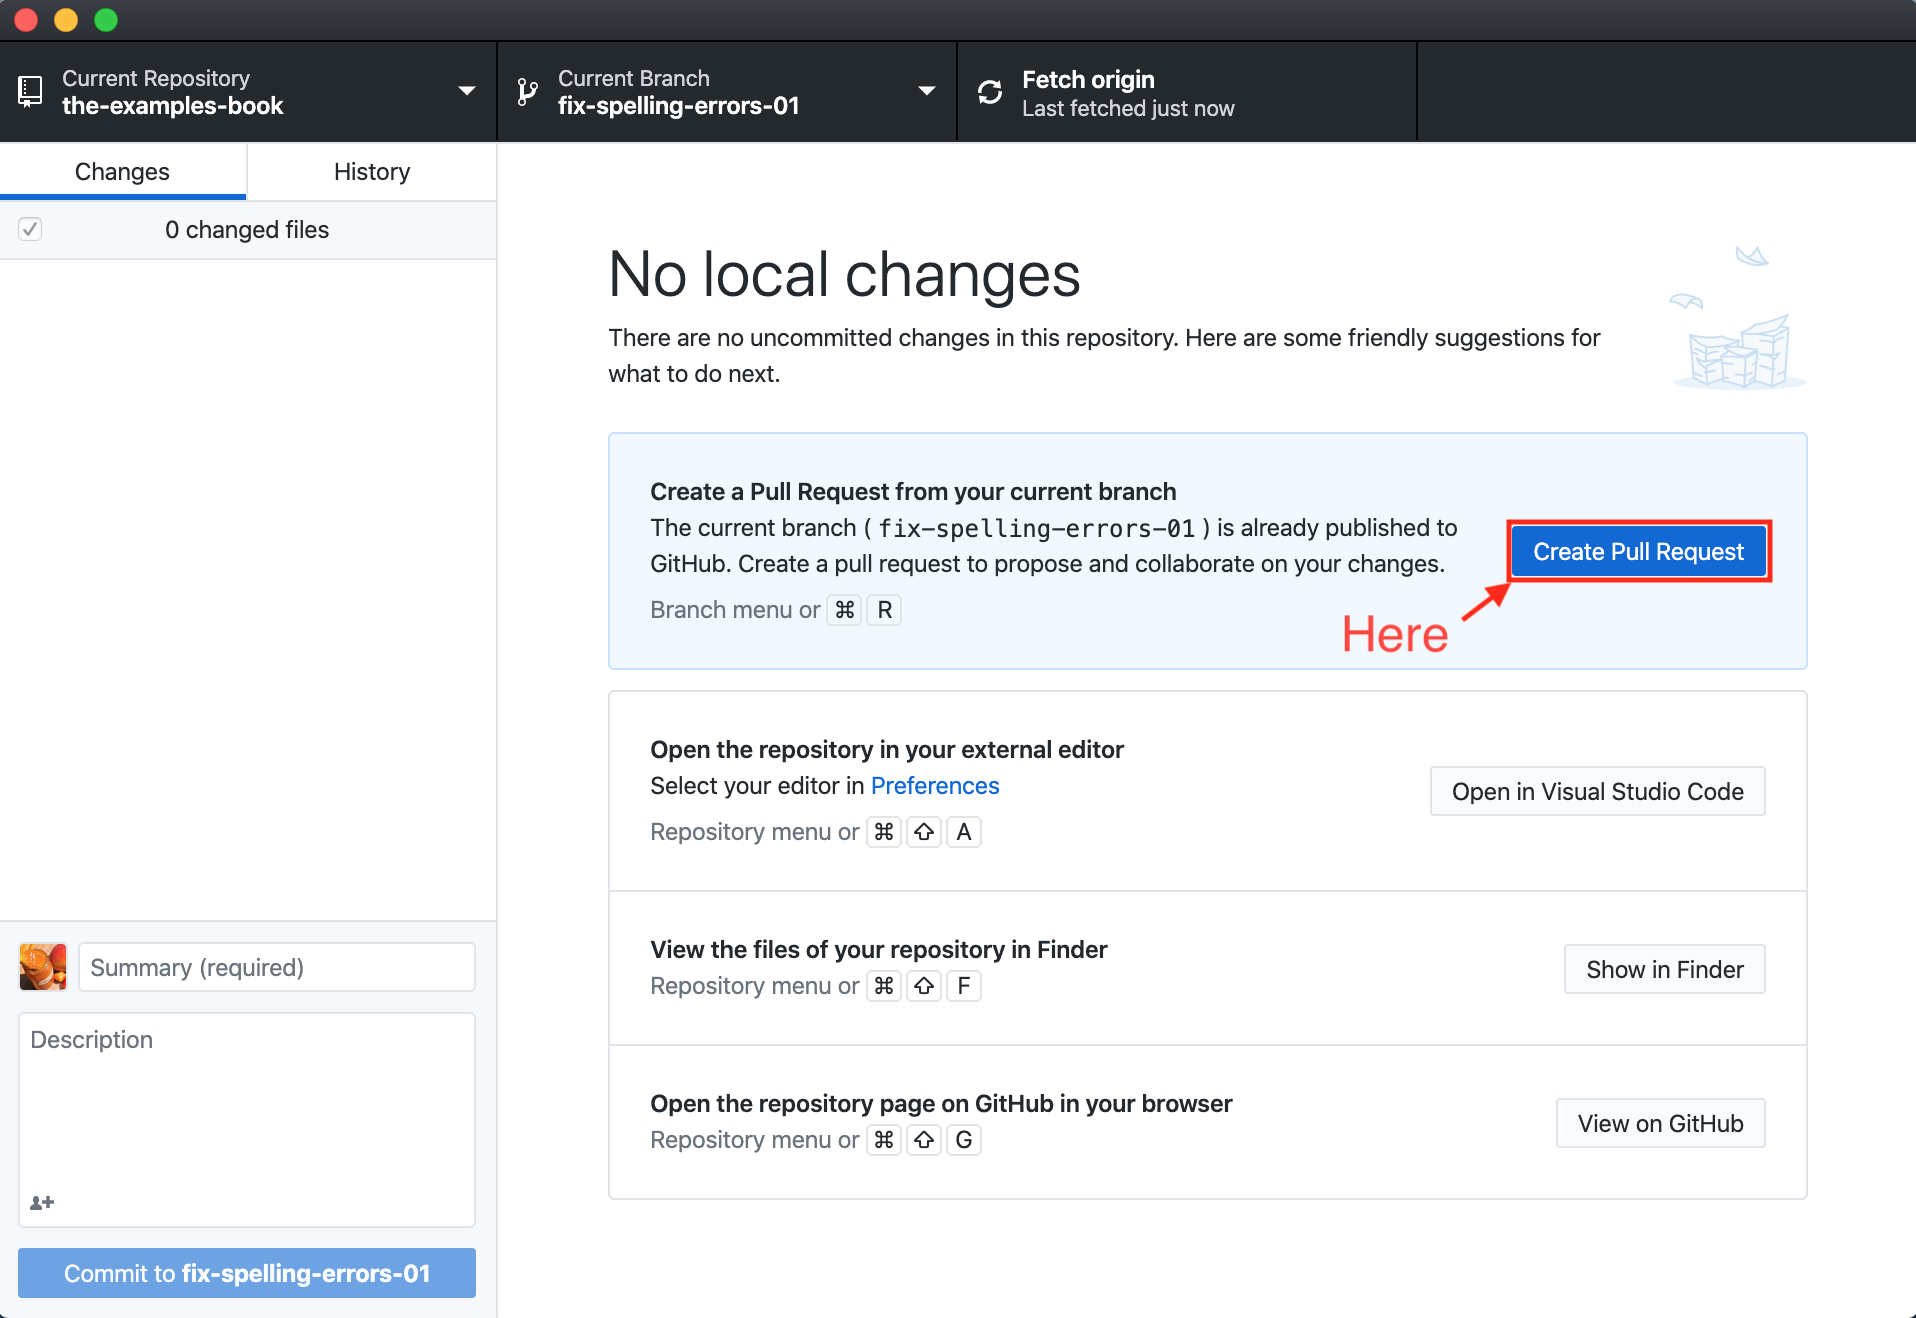
\includegraphics{./images/gh-desktop-12.png}
\caption{}
\end{figure}

\begin{enumerate}
\def\labelenumi{\arabic{enumi}.}
\setcounter{enumi}{19}
\tightlist
\item
  At this point in time, the repository owners will receive a
  notification and will check and potentially merge the changes into the
  \texttt{master} branch. © 2020 GitHub, Inc. Terms Privacy Security
  Status Help Contact GitHub Pricing API Training Blog About
\end{enumerate}

\end{document}
